\documentclass[a4paper]{report}
\usepackage{apacite}
\usepackage{graphicx}
\usepackage{algorithm}
\usepackage{algcompatible}
\usepackage[section]{placeins}
\graphicspath{{Images/}}
\setlength\parindent{0pt}

\makeatletter
\AtBeginDocument{%
	\expandafter\renewcommand\expandafter\subsection\expandafter{%
		\expandafter\@fb@secFB\subsection
	}%
}
\makeatother

\begin{document}
	%------------------------Cover-------------------------------------------------------------
	\begin{titlepage} 
		\newcommand{\HRule}{\rule{\linewidth}{0.5mm}}
		
		\center 
		
		\textsc{\large Project 1.1 - Block 3}\\[0.5cm] 
		
		\HRule\\[0.4cm]
		
		{\huge\bfseries Compute chromatic numbers}\\[0.4cm] 
		
		\HRule\\[1.5cm]
		
		\textsc{\large Group 10}\\[0.5cm]

		\begin{minipage}{0.6\textwidth}
			\begin{flushleft}
				Tu Anh Dinh\\Michal Jarski\\Louis Mottet
			\end{flushleft}
		\end{minipage}
		~
		\begin{minipage}{0.3\textwidth}
			\begin{flushleft}
				Vaishnavi Velaga\\Rudy Wessels\\Oskar Wielgos
			\end{flushleft}
		\end{minipage}
		
		\vspace{2cm}
		
		Submited: Wednesday January 23, 2019
		
		
	\end{titlepage}
	
	
	
	
	
	%-------------------Title page-----------------------------------------------------------
	\begin{titlepage} 
		\newcommand{\HRule}{\rule{\linewidth}{0.5mm}} 
		
		\center
		
		\textsc{\LARGE Maastricht University}\\[1.5cm]
		
		\textsc{\Large Department of Data Science and Knowledge Engineering}\\[0.5cm] 
		
		\textsc{\large Project 1.1 - Block 3}\\[0.5cm] 
		
		\HRule\\[0.4cm]
		
		{\huge\bfseries Compute chromatic numbers}\\[0.4cm] 
		
		\HRule\\[1.5cm]
		
		\textsc{\large Group 10}\\[0.5cm]
		
		\begin{minipage}{0.6\textwidth}
			\begin{flushleft}
				Tu Anh Dinh\\Michal Jarski\\Louis Mottet
			\end{flushleft}
		\end{minipage}
		~
		\begin{minipage}{0.3\textwidth}
			\begin{flushleft}
				Vaishnavi Velaga\\Rudy Wessels\\Oskar Wielgos
			\end{flushleft}
		\end{minipage}
	
		 \vspace{1cm}
		Submited: Wednesday January 23, 2019
		\vspace{3cm}
		\begin{flushleft}
			Project coordinator: Prof. Jan Paredis
		\end{flushleft}
		
	\end{titlepage}
	
	%-----------------------------------------------------------------------------
	\chapter*{Preface}
	\pagenumbering{gobble}

	\addcontentsline{toc}{chapter}{Preface}
	This report is a part of the outcomes of our work for project 1.3: Graph Coloring. It can be used as a guideline to partially solve the non-deterministic polynomial-time hard problem of finding the chromatic number of a graph.
	
%	This report is about graph-coloring(Vertices Coloring ). Graph-Coloring is one of the important topic of graph theory. Task of the project is to compute chromatic number, upper and lower bounds of the given 20 graphs and make different experiments and note down the results of the experiments. This report consist of 6 Chapters. First Chapter is all about brief introduction to Graph- Coloring with few properties, examples and uses .Second Chapter is all about different algorithms like Greedy Algorithm to find upper bound of the graph, Genetic Algorithm to find Chromatic Number of the graph and few other algorithms like Brute force search, Breadth-first search etc. Chapters 3,4 and 5 are about Experiments and their results. Last Chapter would be about the conclusion of the report. 
	
	%-----------------------------------------------------------------------------
	\chapter*{Summary}
	\addcontentsline{toc}{chapter}{Summary}
	This project gives an answer for the question of finding the smallest range of the chromatic number of a graph. The methods used are graph decomposition, greedy algorithm, identifying special cases of graphs, brute-force algorithm and genetic algorithm. This approach gives decent results on small graphs and graphs with special structures. However, the results are unpredictable for large arbitrary graphs.
	
	%-----------------------------------------------------------------------------
	\tableofcontents
	
%	\chapter*{Abbreviations and symbols}
%	\addcontentsline{toc}{chapter}{List of abbreviations and symbols}

	
	%-----------------------------------------------------------------------------
	\chapter{Introduction}
	\pagenumbering{arabic}
	
	A graph is a set of vertices connected by edges. In this project, the input graphs are undirected graph, where the edges have no orientation. In addition, a vertex must not connected to itself and the number of edges between two vertices must not exceed 1. \\
	
	Graph coloring is coloring the vertices of a graph such that no two adjacent vertices share the same color. Graph coloring is one of the important topic of graph theory and is used in real time applications of computer science and it is used in various research areas of computer science such as data mining, networking etc.\\
	
	The smallest number of colors used in graph coloring is called the chromatic number. A lower bound of a graph is a number that is less than or equal to the chromtic number, while an upper bound is a number that is greater than or equal to the chromtic number. The purpose of this project is to find the closest upper bound, lower bound and, if possible, the chromatic number of a graph.\\
	
	The rest of the report is divided as follows. Chapter 2 is about the methods used to compute the upper bound, lower bound and the chromatic number of a graph. Different algorithms are used: graph decomposition, greedy algorithm, identifying special cases of graphs, brute-force algorithm and genetic algorithm. Chapters 3,4 and 5 are about experiments and their results. In the last chapter, the whole project will be concluded.
	
	\chapter{Methods}
	This chapter describes the methods used for finding the lower bound, upper bound and if possible, the chromatic number of a graph. 
	\section{Overview}
	Given the limitation on execution time (2 minutes for each graph), methods that give out results fast are executed first. Algorithm \ref{alg:overview} describes the general work flow.\\
	\begin{algorithm}
		\caption{General work flow}
		\label{alg:overview}
		\begin{algorithmic}[1]
			\REQUIRE a graph
			\STATE upperbound = greedyUpperbound(graph)
			\STATE subgraphs = decompose(graph)
			\FORALL{subgraphs} 
				\STATE subUpperbound =  greedyUpperbound(subgraph)
				
				\STATE//Check all special cases
				\IF{subgraph has no vertex} 
					\STATE chromaticNumber of subgraph = 0
					\STATE Go to the next subgraph
				\ENDIF
				\IF{subgraph has no edge} 
				\STATE chromaticNumber of subgraph = 1
				\STATE Go to the next subgraph
				\ENDIF
				\IF{subgraph is bipartite} 
				\STATE chromaticNumber of subgraph = 2
				\STATE Go to the next subgraph
				\ENDIF
				\IF{subgraph is odd cycle} 
				\STATE chromaticNumber of subgraph = 3
				\STATE Go to the next subgraph
				\ENDIF
				\IF{subgraph is complete graph} 
				\STATE chromaticNumber of subgraph = number of vertices
				\STATE Go to the next subgraph
				\ENDIF
				\IF{subgraph is wheel graph} 
					\IF{number of vertices is odd} 
					\STATE chromaticNumber of subgraph = 3
					\STATE Go to the next subgraph
					\ELSE
					\STATE chromaticNumber of subgraph = 4
					\STATE Go to the next subgraph
					\ENDIF
				\ENDIF
				\STATE subLowerbound = 3
				\IF{subUpperbound = subLowerbound} 
				\STATE chromaticNumber of subgraph = 3
				\STATE Go to the next subgraph
				\ENDIF
				
				\STATE//Run brute-force
				\IF{number of vertices $<=$ 20} 
				\STATE chromaticNumber of subgraph = BruteForce(subgraph)
				\ENDIF 
			\ENDFOR

			\algstore{myalg}
			\end{algorithmic}
		\end{algorithm}

		\begin{algorithm}                     
			\begin{algorithmic} [1]     
			\algrestore{myalg}

			\STATE newUpperbound = max(subUpperbounds)
			
			\IF{newUpperbound $<$ upperbound} 
			\STATE //Update upper bound
			\STATE upperbound = newUpperbound 
			\ENDIF
			
			\STATE lowerbound = max(subLowerbounds)
			
			\IF{has found all chromatic numbers of subgraphs} 
			\STATE chromatic number = max(chromatic numbers of subgraphs)
			\ELSE
			\STATE lowerbound = max(chromatic numbers of subgraphs)
			\ENDIF
			
			\STATE geneticAlgorithm(graph)
		\end{algorithmic}
	\end{algorithm}
	First, a greedy algorithm is run on the given graph to calculate the upper bound (line 1). Then, the given graph is decomposed to disconnected subgraphs. For each subgraph, the greedy algorithm is run again to find the upper bound (line 2). Then all special cases are checked to see if the chromatic number of the subgraph can be concluded immediately(line 3 - 34). The special cases are listed below: 
	\begin{itemize}
		\item No-vertex graph: chromatic number is 0
		\item No-edge graph: chromatic number is 1
		\item Bipartite graph: chromatic number is 2
		\item Odd cycle: chromatic number is 3
		\item Complete graph: chromatic number is the number of vertices
		\item Wheel graph: if the number of vertices is odd, then the chromatic number is 3, otherwise the chromatic number is 4
	\end{itemize}
	In line 35, if a subgraph is none of the special cases, the lower bound of the subgraph is 3, since the first three cases have covered all graphs where the chromatic number is below 3. If the upper bound is also 3, then the chromatic number of the subgraph is 3. \\
	If the chromatic number of a subgraph still cannot be concluded then a brute-force algorithm is used (line 41 - 43). However, only subgraphs with number of vertices below 20 are proccessed with the brute-force algorithm, since the brute-force algorithm normally takes longer than 2 minutes to execute on bigger graphs. \\
	
	After proccessing on the subgraphs, the upper bound, the lower bound and possibly the chromatic number of the original graph can be concluded. The biggest upper bound among the subgraphs is the upper bound of the original graph (line 45). This new upper bound is then compared to the previously computed upper bound in line 1 to output the better one. Similarily, the biggest lower bound among the subgraphs is a lower bound of the original graph (line 50). \\
	If the chromatic numbers of all subgraphs have been found, then the chromatic number of the original graph is the biggest chromatic number among the subgraphs (line 52). If it is not the case, then the biggest chromatic number found on the subgraphs is another lower bound for the original graph (line 54).\\
	Finally, in line 56, genetic algorithm is used to bring the upper bound closer to the chromatic number. Genetic algorithm is run last because there is no guarantee on its execution time.\\
	
	The algorithm for each method is described in the next sections of this chapter.
	

		\section{Graph decomposition}
		One graph can contain multiple disconnected parts, which can be considered as independent subgraphs (Figure \ref{fig:decompose}). Decomposing the graph will allow other methods to work on smaller graphs. Algorithm \ref{alg:decompose} describes the method for decomposing a graph into subgraphs, where each subgraph is a fully connected graph.\\
		
		\begin{figure}[h]
			\centering
			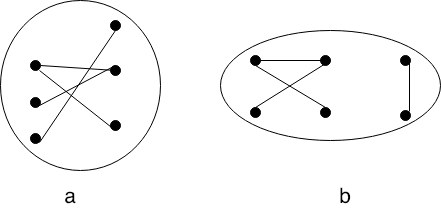
\includegraphics[width=50mm,scale=0.5]{figures/DecomposedGraph.png}
			\caption{A graph (a) before decomposed and (b) after decomposed}
			\label{fig:decompose}
		\end{figure}
	
		\begin{algorithm}
			\caption{Decomposing a graph}
			\label{alg:decompose}
			\begin{algorithmic}[1]
				\REQUIRE a graph
				\STATE Create listOfVertices 
				\STATE listOfVertices.add(all vertices in the graph)
				\WHILE{listOfVertices is not empty}
				\STATE Create a new subgraph
				\STATE Create a new uncheckedList
				\STATE subgraph.add(firstVertex in listOfVertices )
				\STATE uncheckedList.add(firstVertex in listOfVertices)
				\STATE listOfVertices.remove(first element)
				\WHILE{uncheckedList is not empty} 
				\STATE checkingVertex = first vertex in the uncheckedList
				\FORALL{neighbors of checkingVertex} 
				\IF{neighbor is not in subgraph} 
				\STATE uncheckedList.add(neighbor)
				\STATE subgraph.add(neighbor)
				\ENDIF
				\STATE listOfVertices.remove(neighbor)
				\ENDFOR
				\STATE Remove checkingVertex from uncheckedList
				\ENDWHILE
				\STATE Convert subgraph to standard form
				\STATE subgraphs.add(subgraph)
				\ENDWHILE
				\STATE \textbf{return} subgraphs
				
			\end{algorithmic}
		\end{algorithm}
		The algorithm is based on breadth-first search. A unchecked-list stores the vertices whose neighbors are not yet added to the current expanding subgraph. In line 6 and 7 the first vertex is added to a subgraph and the unchecked list. Then all the neighbors of the vertex are added to the subgraph and the unchecked list, and the first vertex of the unchecked list is removed (line 9 - 19). To avoid loops, only vertices not in the subgraph are added. The same is done for all vertices in the unchecked list, until the list is empty. The process is repeated until all vertices in the original graph are classified into subgraphs.\\
		Note that the vertices of the input graphs for this project are represented by successive numbers. All algorithms are implemented based on this data structure. Therefore, after classifying the vertices into subgraphs, each subgraph is then converted to the standard form, where the indexes of vertices are successive numbers (line 20).
		
		\section{Greedy algorithm}
		Greedy algorithm \cite{greedy} provides an efficient way of coloring a graph. However, it does not guarantee that the coloring is optimal. Therefore, it can be used to calculate a upper bound. Algorithm \ref{alg:greedy} describes this method.\\
		\begin{algorithm}
			\caption{Greedy algorithm for upper bound}
			\label{alg:greedy}
			\begin{algorithmic}[1]
				\REQUIRE a graph
				\STATE Sort vertices in non-increasing order of constraints
				\STATE Create availableColors list
				\FORALL{vertices}
					\FORALL{colors in availableColors}
					\IF{color is valid for vertex}
					\STATE Assign the color for the vertex
					\STATE break
					\ENDIF
					\ENDFOR
					\IF{The vertex is still not colored}
					\STATE Create a new color
					\STATE Assign the new color for the vertex
					\STATE Add the new color to availableColors list
					\ENDIF
				\ENDFOR
				\STATE \textbf{return} size of availableColors list
			\end{algorithmic}
		\end{algorithm}
		First, the vertices are sorted based on their constraints (line 1). The constraint of a vertex is the number of other vertices connected to that vertex. Optimized bubble sort \cite{bubblesort2019} is used in this step. The vertex with more neighbors will be colored first.\\
		A list is used to store available colors. When coloring a vertex, the available colors is reused as much as possible (line 4-9). If none of the available colors is valid to color that vertex, then a new color is generated and added to the available list (line 10-14). When the graph is fully colored, the number of colors in the available list is returned.\\
		
		\section{Lower bound}
		
		\section{Special cases}
			\subsection{Bipartite}
			The formal definition of a bipartite graph is: \\
			"A bipartite graph, also called a bigraph, is a set of graph vertices decomposed into two disjoint sets such that no two graph vertices within the same set are adjacent." \cite{bipartiteDef} \\
			The chromatic number of a bipartite graph is 2. Algorithm \ref{alg:bipartite} \cite{bipartite} describes the steps to test weather a graph is bipartite, using breadth-first search. \\
			
			\begin{figure}[h]
				\centering
				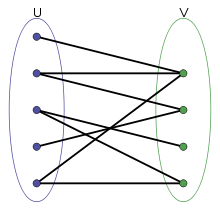
\includegraphics[width=50mm,scale=0.5]{figures/bipartite.png}
				\caption{An example of bipartite graphs. This figure is from \protect\cite{bipartiteFig}}
				\label{fig:bipartite}
			\end{figure}
			
			\begin{algorithm}
				\caption{Bipartite testing}
				\label{alg:bipartite}
			
				\begin{algorithmic}[1]
					\REQUIRE a graph
					\STATE Create unchecked list
					\STATE unchecked.add(first vertex)
					\STATE Assign color 1 to the first vertex
					\WHILE{The graph is not fully colored}
					\WHILE{unchecked list is not empty}
					\STATE checkingVertex = unchecked.getFirstElement()
					\STATE unchecked.removeFistElement
					\FORALL{neighbors of checkingVertex}
					\IF{neibor not yet colored}
					\STATE Assign the opposite color of checkingVertex's color to neighbor
					\STATE unchecked.add(neighbor)
					\ELSIF{neighbor has invalid color}
					\STATE \textbf{return} false
					\ENDIF
					\ENDFOR
					\ENDWHILE
					\ENDWHILE
					\STATE \textbf{return} true
				\end{algorithmic}
			\end{algorithm}
			 Two colors, represented by 1 and -1, are used to color the graph. A unchecked list stores the vertices whose neighbors are not yet considered. First, the color 1 is assigned to the first vertex and the first vertex is added to the unchecked list (line 2-3). Then, all its neighbors are considered and the vertex itself is removed from the unchecked list. For each neighbor, if the neighbor has not been colored then it is assigned with the oposite color (line 10). If the neighbor has been colored, then we check if it is a valid coloring. If the coloring is invalid, the graph is not bipartite (line 12-13). The same is done for all elements in the unchecked list, until the list is empty. The process is repeated until all vertices in the graph are colored. If the graph is successfully colored, then it is bipartite.
			\subsection{Odd cycle}
			An odd cycle is a cycle with an odd number of edges and vertices (Figure \ref{fig:oddcycle}). The chromatic number of an odd cycle graph is 3. \\
			
			\begin{figure}[h]
				\centering
				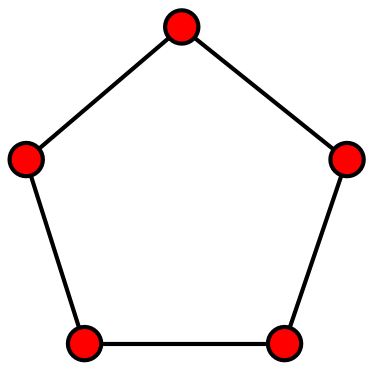
\includegraphics[width=50mm,scale=0.5]{figures/cycle.png}
				\caption{An example of odd cycle graphs. This figure is from \protect\cite{cycleFig}}
				\label{fig:oddcycle}
			\end{figure}
		
			The method for testing if a graph is an odd cycle checks for three condition:
			\begin{itemize}
				\item The number of vertices is equal to the number of edges
				\item Every vertex has two edges
				\item The number of vertices is odd
			\end{itemize}
			A graph is an odd cycle graph if and only if all three conditions are satisfied.
			
			\subsection{Complete graph}
			A complete graph (Figure \ref{fig:complete}) is a graph where every vertex is connected to all other vertices. The chromatic number of a complete graph is the number of vertices. The method checks weather a graph has the above conditions to determine if it is a complete graph.
			\begin{figure}[h]
				\centering
				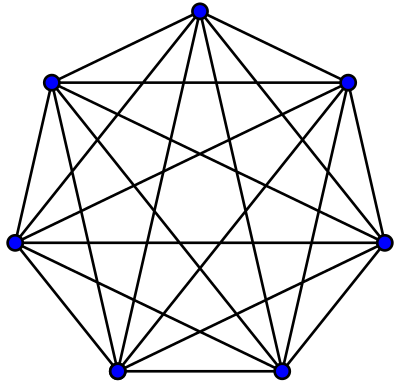
\includegraphics[width=50mm,scale=0.5]{figures/complete.png}
				\caption{An example of complete graphs. This figure is from \protect\cite{completeFig}}
				\label{fig:complete}
			\end{figure}
			
			\subsection{Wheel graph}
			A wheel graph (Figure \ref{fig:wheel}) is formed by connecting a single vertex to all vertices of a cycle.
		
			\begin{figure}[h]
				\centering
				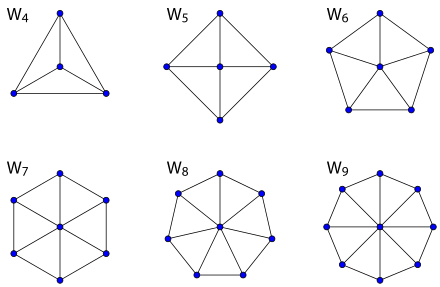
\includegraphics[width=50mm,scale=0.5]{figures/wheel.png}
				\caption{Examples of wheel graphs. This figure is from \protect\cite{wheelFig}}
				\label{fig:wheel}
			\end{figure}
			
			The method used to check whether a graph is a wheel graph is as follows. First, every vertex is checked to see if it is connected to all the  remaining vertices of the graph. If that condition is satisfied, then the vertex is the center. Next, the center is removed from the graph. If the remaining graph is a cycle, then the original graph is a wheel graph.
			If the graph is a wheel graph with odd number of vertices, then chromatic number is 3. Otherwise, if the graph is a wheel graph with even number of vertices, then chromatic number is 4.
			
			
		\section{Brute-force algorithm}
		The brute-force algorithm simply generates every possible coloring and checks if it's a valid one. In case the coloring is valid, the algorithm terminates with a possibilty of returning an array of colors assigned to each node and the chromatic number. In order to check the validity of coloring, it utilizes isValid algorithm, that iterates through the array representing nodes' colors and searches for a conflict (two adjacent/connected nodes having assigned the same color). If found, false is being returned instantly, meaning certain coloring is not a valid one.\\
		
		Brute-force is based on raw computetional power, thus making it heavily dependent on the hardware that runs it. Finding the chromatic number is GUARANTEED sooner or later. However in reality, its use is limited to graphs not bigger than 20 nodes, and even then, depending yet on how the vertices are being connected.\\
		
		Algorithms calculating lower bound or applying pruning, might futher optimize it, reducing the time needed to find the chromatic number. \\
		
		Implementing a greedy-type brute-force could also bring significant improvements on effectivness and execution time, but on the other hand, causing a risk of omitting the right coloring and eventually not finding the chromatic number, but only its approximation.	
			
		\section{Genetic algorithm}
%			\subsection{Fitness function}
%			\subsection{Selection method}
%			\subsection{Crossover}
%			\subsection{Mutation}
		The genetic algorithm is an algorithm for calculating the upper bound together with working its way down to finding lower and better upper bounds for a particular graph. It starts with creating a population of individuals each containing a randomly colored version of the selected graph. The size of this population can be set to any number preferred. Once the population is created it assigns a fitness (which is a real number between 0 and 1) to each individual based on the number of incorrect edges. Following up the individuals are sorted by fitness from high to low (1$>$0), at which it becomes clear what part of the population has the highest correctness of coloring.\\
		
		After the individuals are sorted the selection method picks out the “parents” for the next generation through an elitist approach. These parents are utilized for the crossover method creating combinations of two of the parents until there are enough new individuals for the next generation with equal size to the previous one. Afterward, the mutation method, depending on the extent of the mutation rate, will mutate some individuals’ coloring of the graph to achieve possibly better results. By results is meant, individuals with higher fitness.
\\
		
		Lastly, this process runs over several generations/populations through a loop till the algorithm finds an individual with fitness “1” (no incorrect edges). When this is the case, the new upper bound will be printed in the command prompt based on how many colors were used to achieve this solution. Following up the entire process starts over with one less color, so that the upper bound will be lower after each successful finding.
		
		
		
	\chapter{Experiments}
	The experiment is set up to run on the given 20 graphs.
	\chapter{Results}
		\begin{table} [h!]
		\begin{center}
			\begin{tabular}{| c | c | c | c |}
				\hline
				Graph no. & Upper bound & Lower bound & Chromatic number  \\
				\hline
				1 & 3 & x & 3 \\
				\hline
				2 & 5 & 3 & x \\
				\hline
				3 & 8 & 6 & x \\
				\hline
				4 & 7 & 3 & x \\
				\hline
				5 & 4 & x & 2 \\
				\hline
				6 & 3 & x & 3 \\
				\hline
				7 & 12 & 3 & x \\
				\hline
				8 & 98 & 3 & x \\
				\hline
				9 & 6 & 3 & x \\
				\hline
				10 & 3 & x & 3 \\
				\hline
				11 & 15 & 3 & x \\
				\hline
				12 & 3 & x & 2 \\
				\hline
				13 & 14 & 3 & x \\
				\hline
				14 & 5 & 3 & x \\
				\hline
				15 & 10 & 3 & x \\
				\hline
				16 & 4 & 3 & x \\
				\hline
				17 & 8 & 3 & x \\
				\hline
				18 & 11 & 3 & x \\
				\hline
				19 & 11 & 3 & x \\
				\hline
				20 & 9 & 3 & x \\
				\hline
			\end{tabular}
		\end{center}
		\caption{Results on the given 20 graphs}
		\label{Mu table}
	\end{table}

	\chapter{Discussion}
	
	\chapter{Conclusion}
	
	
	\bibliographystyle{apacite}
	\bibliography{references}
	
%	\appendix
%	\chapter*{Appendix}
%	\addcontentsline{toc}{chapter}{Appendix}
\end{document}